{\let\clearpage\relax \chapter{White box identification}}
\section{Detached system: cart and springs identification}
\label{sec:cart_detached_id}
To accurately identify the mass of the cart and the stiffness/damping of the spring ,the motor was detached from the cart, in order to reduce influence of friction due to the pinion and rack. \\ \\
So we obtain a system like the one considered in figure \ref{fig:cart_detached_motor}.

\begin{figure}[!h]
\centering
\begin{tikzpicture}[every node/.style={draw,outer sep=0pt,thick}]
\tikzstyle{spring}=[thick,decorate,decoration={zigzag,pre length=0.3cm,post length=0.3cm,segment length=6}]
\tikzstyle{damper}=[thick,decoration={markings,  
  mark connection node=dmp,
  mark=at position 0.5 with 
  {
    \node (dmp) [thick,inner sep=0pt,transform shape,rotate=-90,minimum width=15pt,minimum height=3pt,draw=none] {};
    \draw [thick] ($(dmp.north east)+(2pt,0)$) -- (dmp.south east) -- (dmp.south west) -- ($(dmp.north west)+(2pt,0)$);
    \draw [thick] ($(dmp.north)+(0,-5pt)$) -- ($(dmp.north)+(0,5pt)$);
  }
}, decorate]
\tikzstyle{ground}=[fill,pattern=north east lines,draw=none,minimum width=0.75cm,minimum height=0.3cm]

 
\begin{scope}[xshift=7cm]
\node (M) [minimum width=1cm, minimum height=2.5cm] {$M$};

\node (ground) [ground,anchor=north,yshift=-0.25cm,minimum width=1.5cm] at (M.south) {};
\draw (ground.north east) -- (ground.north west);
\draw [thick] (M.south west) ++ (0.2cm,-0.125cm) circle (0.125cm)  (M.south east) ++ (-0.2cm,-0.125cm) circle (0.125cm);

\node (wall) [ground, rotate=-90, minimum width=3cm,yshift=-3cm] {};
\draw (wall.north east) -- (wall.north west);

\draw [spring] (wall.170) -- ($(M.north west)!(wall.170)!(M.south west)$) node [draw=none,midway,above=0.3cm] {$k$};
\draw [damper] (wall.10) -- ($(M.north west)!(wall.10)!(M.south west)$) node [draw=none,midway,above=0.3cm] {$c$};

\draw [-latex,ultra thick] (M.east) ++ (0.2cm,0) -- +(1cm,0) node [draw=none, midway,above=0.3cm] {$x$};
\end{scope}
\end{tikzpicture}
\caption{Cart detached from the motor diagram.}
\label{fig:cart_detached_motor}
\end{figure}

The differential equation governing this system is given by:
$$M\ddot{x}+c_i\dot{x}+k_i x = f(t)$$
where $M$ [\SI{}{\kilo \gram}] is the total mass of the system  , $c_i$ [\SI{}{\newton \second \per \meter }] comprehends the damping of the $i$-eth spring and the viscous damping of the sliding guide. Finally $k_i$ [\SI{}{\newton \per \meter}] is the stiffness of the $i$-eth spring, and $f(t)$ represents external forces acting on the system (such as non-linear friction components). 
\\ \\
\subsection{Experiment description}
For each spring we conducted 2 experiments, one without any load and one with a load of $0.986$ [\si{\kg}], each repeated 3 times. To accurately identify the mass of the cart and the stiffness/damping of the spring ,the motor was detached from the cart, in order to reduce influence of friction due to the pinion and rack. \\\\
For each experiment the  cart was released from an initial condition $x(0) =x_0 \neq 0$ and $0$ velocity,  such that the force that the spring was exerting on the cart was sufficient enough to  make negligible the very small component of the static friction acting on the cart. \\ Notice that the initial condition differs for each spring since the stiffness is very different for each spring. \\\\
If we neglect the external forces acting on the cart, which are negligible since they are small non-linear components, then the system considered is:
\begin{equation} \label{eq:cart_detached_motor}
\begin{cases}
M\ddot{x}+c_i\dot{x}+k_i x = 0 \\
x(0) \in [1,3] \SI{}{\cm} \\
\dot{x}(0)=0
\end{cases}
\end{equation} \\ \\
Then data regarding the position of the cart is collected, and from that data the pulsation, damping ratio, mass and stiffness are retrieved.


\subsection{Experiment analysis}
Using \ref{eq:cart_detached_motor} the response in time can be obtained by using the Laplace transform. Let $X(s)$ be the Laplace transform of $x(t)$, then:
$$mX(s)(s^2-x(0)s) +c X(s) (s-x(0)) +kX(s)=0$$
and:
$$X(s) = x(0) \frac{(ms+c)}{ms^2+cs+k}$$
If we solve in $X(s)$ and then apply the inverse Laplace transform, we obtain the response in time:
$$x(t) = e^{-\xi \omega_0 t}(A\cos(\omega t)+B\sin(\omega t))$$
where $\xi = \frac{c}{2\sqrt{Mk}}, \omega_0 = \sqrt{\frac{k}{M}}, \omega = \omega_0 \sqrt{1-\xi^2}$, and $A,B$ depend on $x(0), \xi$. \\ \\
Since the pulsation is the same for both sinusoidal components we have:
$$x(t) = C e^{-\xi \omega_0 t} \sin(\omega t+ \phi)$$
Where  $C= \sqrt{A^2+B^2}, \phi = \arctan(A/B)$.
\\ \\
Knowing those equations we  are able to extract data from the response in the following way:
\begin{itemize}

\item {To measure $\omega$ we can just extract the period $T$:  the difference in time between the first and second peak is taken, and that difference is the period. Then $\omega$ is just $\frac{2\pi}{T}$. We consider only the first and second peak because  at the beginning non-linearities such as static  and coloumb friction are negligible. }

\item {To measure $\xi$ also the first and second peak are considered. Let $t_0, t_1$ be the times at which there is the first and second peak. Notice that $t_0=0, t_1=T$, and $x(T)= Ae^{-\xi \omega_0 T}$.\\
Then, consider:
$$\log \Big(\frac{x(0)}{x(T)}\Big) =  \log(e^{\xi \omega_0 T}) = \xi \omega_0 T = \frac{\xi}{\sqrt{1-\xi^2}} 2\pi$$
Then $$\xi = \frac{a}{\sqrt{a^2+1}}, \quad a = \frac{1}{2\pi}\log \Big(\frac{x(0)}{x(T)}\Big)$$
Once $M,k$ are known we can calculate the damping from $c= 2\xi \sqrt{Mk}$. Observe that for $a \sim 0 \Rightarrow \xi \sim a$. \\ Since damping
}

\item {To identify each spring and the mass of the cart we made use of the fact that the we have two type of experiments for each spring: one without any load, and one with a load of  $0.986$ \SI{}{\kilo\gram}. We obtain a system of linear equations:
$$
\begin{cases}
\frac{k_i}{m_c+m_l} = \omega_l^2 \\
\frac{k_i}{m_c} = \omega_{nl}^2 \\
\end{cases}
$$
Where $m_c$ is the mass of the cart, $m_l$ the mass of the load, $\omega_l$ the pulsation of the system with the load, $\omega_{nl}$ the pulsation of the system without the load. It's a system with two unknowns ($k_i, m_c$) and two equations, so we can solve it. We can rewrite it in matrix form:
$$\begin{bmatrix}
1  && - \omega_l^2 \\
1 && -\omega_{nl}^2
\end{bmatrix}  
\begin{bmatrix}
k_i \\ m_c
\end{bmatrix}  
=\begin{bmatrix}
w_l^2 m_l \\
0
\end{bmatrix}  
$$
and solve for ($k_i, m_c$).
}


\end{itemize}
\subsection{Experiment results}
Since there are $3$ springs let's denote the set of springs as $K=\{k_l, k_m, k_h\}$ where \emph{l} stands for low, \emph{m} for medium and \emph{h} for high. In a similar manner we define the various pulsation: for example $\omega_{m-nl}$ is the pulsation for the system with spring $k_m$ and no load.
\\ \\ 
\paragraph{Pulsation}
In the table below are shown the various mean of the pulsation and their relative standard deviation:
\begin{table}[!h]
\centering

\label{table: cart_detached_omega}
\begin{tabular}{|l|l|l|l|}
\hline
{(\textbf{$\omega_{avg}$} [\SI{}{\radian \per \second}],$\omega_{std}$ [\SI{}{\radian \per \second}])} & \textbf{$k_h$} & \textbf{$k_m$}   & \textbf{$k_l$}   \\ \hline
\textbf{with load}         & (21.2989, 0)    & (14.2800, 0.0671) & (10.6495, 0)      \\ \hline
\textbf{with no load}      & (34.9066, 0)    & (23.7101, 0.1792) & (17.6991, 0.1005) \\ \hline
\end{tabular}
\caption{Pulsation of the cart detached from the motor. Various configuration are shown (with a load of $0.986$ [\SI{}{\kilo \gram}] and no load) for the various springs. }
\end{table} \\ \\
It's interesting to note that even if we considered to average all the periods by considering the various peaks of the signal, and not only the first two peaks, we would have obtained the same results. This is an hint of the fact that the principal non-linearity, i.e. coloumb friction, is negligible.

\begin{figure}[!ht]
    \centering
    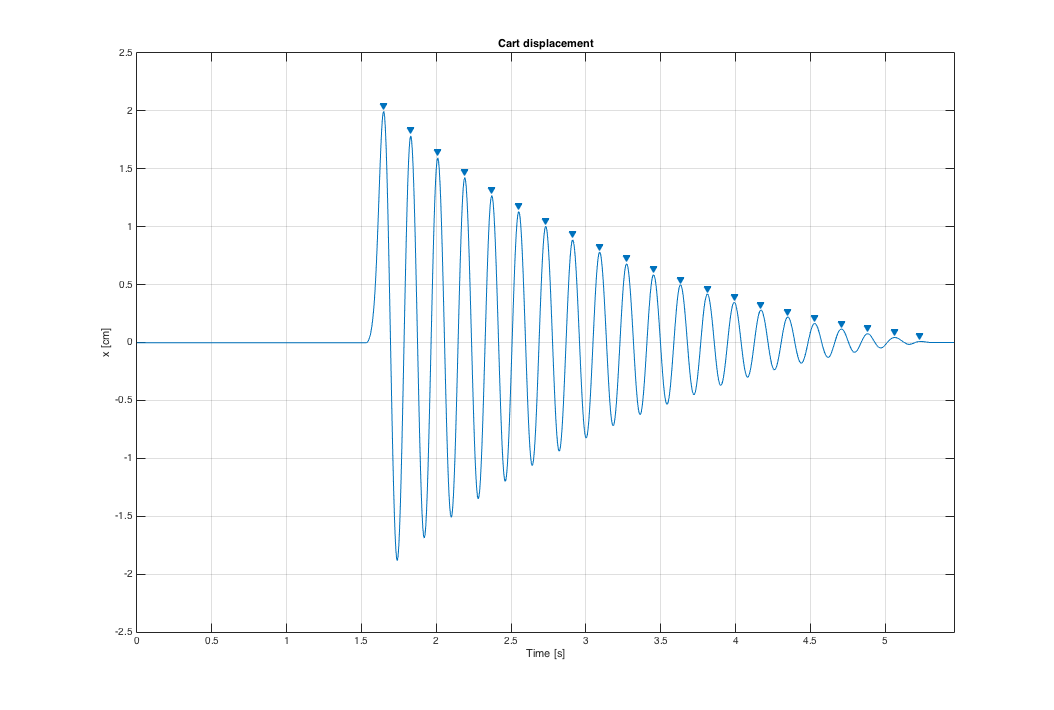
\includegraphics[width=0.5\textwidth]{img/cart_detached_1.png}
    \caption{Displacement of the cart with spring $k_h$ and load $0.986$ [\SI{}{\kilo \gram}].}
    \label{fig:cart_detached_figure}
\end{figure}
\paragraph{Cart mass and springs stiffness}
By using   mean pulsation the resultant average mass of the cart $m_c$ is $0.5685$ [\SI{}{\kilo\gram}] with standard deviation $  0.0141$ [\SI{}{\kilo \gram}]. Results also for the springs are shown in table \ref{table: cart_springs_mass}.
\begin{table}[!h]
\centering
\label{table: cart_springs_mass}
\begin{tabular}{|l|l|l|}
\hline
{\textbf{($k_h$ [\SI{}{\newton \per \metre}], $m_c$ [\SI{}{\kilo \gram}])}} & \textbf{($k_m$ [\SI{}{\newton \per \metre}], $m_c$ [\SI{}{\kilo \gram}])} & \textbf{($k_l$ [\SI{}{\newton \per \metre}], $m_c$ [\SI{}{\kilo \gram}])} \\ \hline
(712.5990, 0.5848)              & (315.5074, 0.5612 )     & (175.2819, 0.5595 )     \\ \hline
\end{tabular}
\caption{Identified springs and cart mass}
\end{table}

\paragraph{Damping and damping ratio}
The mean values for the damping ratio, including their standard deviation, are shown in table \ref{table: cart_detached_dampingratio} for the various springs, with and without a load.
\begin{table}[!h]
\centering

\label{table: cart_detached_dampingratio}
\begin{tabular}{|l|l|l|l|}
\hline
{(\textbf{$\xi_{avg}$},$\xi_{std}$)} & \textbf{$k_h$} & \textbf{$k_m$}   & \textbf{$k_l$}   \\ \hline
\textbf{with load}         & (0.0128,  0.0007 )    & (0.0238, 0.0018) & (0.0346, 0.0036) \\ \hline
\textbf{with no load}      & (0.0179, 0.0025 )    & (0.0301, 0.0013) & (0.0379, 0.0040)      \\ \hline
\end{tabular}
\caption{Damping ratio. Various configuration are shown (with a load of $0.986$ [\SI{}{\kilo \gram}] and no load) for the various springs. }
\end{table}


From the values shown in table \ref{table: cart_detached_damping} it seems that the damping $C$ is function of the mass, in fact we don't obtain the same dampingif we consider the damping ratio with no load or with load. For example consider $k_h$: with a load we obtain $C= 0.0128\cdot2\cdot\sqrt{k_h M}=0.8520$ [\SI{}{\newton \second \per \metre}], without load: $C=0.0179\cdot2\cdot\sqrt{k_h m_c}=0.7206$ [\SI{}{\newton \second \per \metre}]. This is most likely an effect due to friction, and the various damping values are shown in table 
\ref{table: cart_detached_damping}.
\begin{table}[!h]
\centering
\label{table: cart_detached_damping}
\begin{tabular}{|l|l|l|l|}
\hline
{$C$ [\SI{}{\newton \second \per \metre}]} & \textbf{$k_h$} & \textbf{$k_m$}   & \textbf{$k_l$}   \\ \hline
\textbf{with load}         &0.8520    & 1.0542 & 1.1423 \\ \hline
\textbf{with no load}     &0.7206    & 0.8063 & 0.7567      \\ \hline
\end{tabular}
\caption{Damping values. Various configuration are shown (with a load of $0.986$ [\SI{}{\kilo \gram}] and no load) for the various springs. }
\end{table}

We can therefore linearly characterize the damping value as function of the mass centered in $m_c$, for each spring:
$$C(m)=C_{nl}+ \frac{C_{l}-C_{nl}}{m_{l}}(m -m_{c}) = C_{nl} +\alpha (m-m_{c})$$
The different values of $\alpha$, the difference quotient, are shown in table \ref{table: cart_detached_damping_quotient}

\begin{table}[!h]
\centering
\label{table: cart_detached_damping_quotient}
\begin{tabular}{|l|l|l|l|}
\hline
 & \textbf{$k_h$} & \textbf{$k_m$}   & \textbf{$k_l$}   \\ \hline
$\frac{C_{l}-C_{nl}}{m_{l}}$ [\SI{}{\newton \second \per \metre \per \kilo\gram}]       &0.1334   & 0.2514 & 0.3911 \\ \hline
\end{tabular}
\caption{Damping difference quotient. Due to friction damping changes for different weights, we can therefore characterize the damping in a linear way with the formula: $C(m)=C_{nl}+ \frac{C_{l}-C_{nl}}{m_{l}}(m -m_{c})= C_{nl} +\alpha (m-m_{c})$. Values of the difference quotient are shown for the different springs.}
\end{table}


\subsection{Validation}
Validation was done in a similar fashion as the experiments conducted to identify the system parameters. The cart was released from a random initial condition $x_0$  and then released. \\ \\ 
Measurements  were compared with the output smulation of a model constructed from the identified parameters, and results were compared with the cost function defined in \ref{sec:validation_cost_function}.


\begin{figure} [!h]
\begin{minipage}[t]{0.4\textwidth}
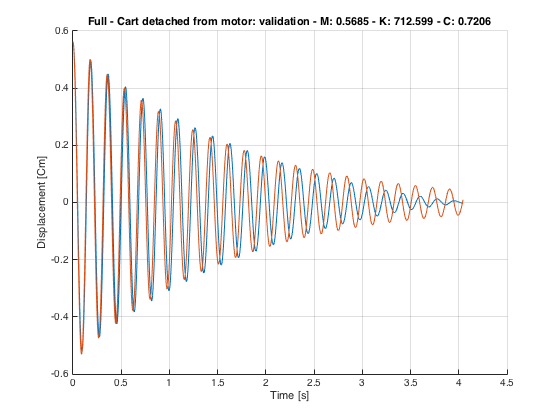
\includegraphics[width=\linewidth]{img/validation_m_kh_full.png}
\caption{Validation test without load and $K_h$.}
\label{fig:val1_1}
\end{minipage}
\hspace{\fill}
\begin{minipage}[t]{0.4\textwidth}
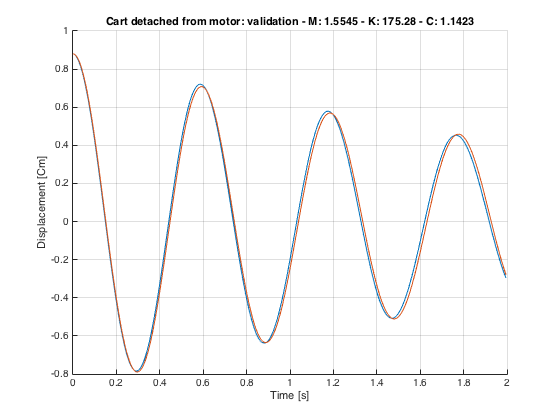
\includegraphics[width=\linewidth]{img/validation_ml_kl_partial.png}
\caption{Validation test without load and $K_l$.}
\label{fig:val1_2}
\end{minipage}

\vspace*{0.5cm} % (or whatever vertical separation you prefer)
\begin{minipage}[t]{0.4\textwidth}
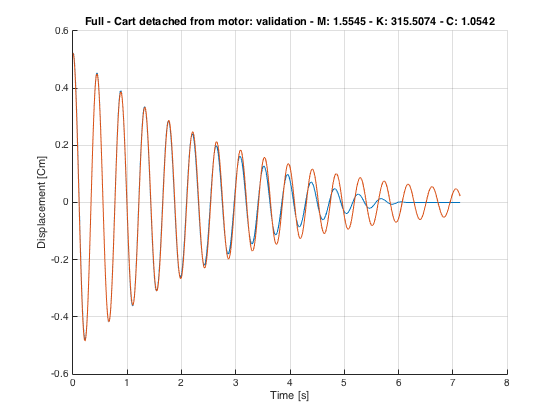
\includegraphics[width=\linewidth]{img/validation_ml_km_full.png}
\caption{Validation test with  load and $K_m$.}
\label{fig:val1_3}
\end{minipage}
\hspace{\fill}
\begin{minipage}[t]{0.4\textwidth}
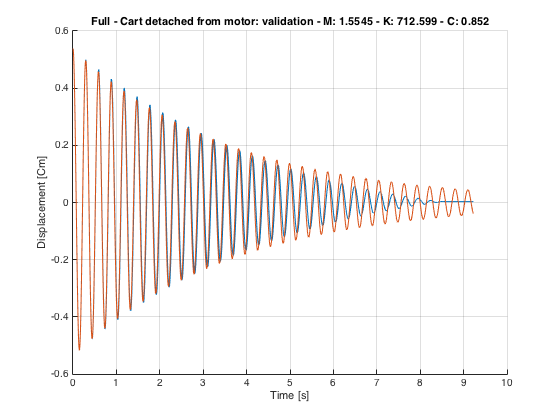
\includegraphics[width=\linewidth]{img/validation_ml_kh_full.png}
\caption{Validation test with  load and $K_h$.}
\label{fig:val1_4}
\end{minipage}
\caption{Validation tests of the cart detached from the motor. In orange the simulated output, in blue the measurement of the validation test. Effect of friction is clearly visible, such as in \ref{fig:val1_3}, where the cart stops after $6$ seconds.}
\label{fig:val1}
\end{figure}

On average, the cost function, on a scale from $0$ to $1$, gave a fit of $ 0.9449$ with standard deviation $0.0263$.
The minimum was $0.8778$, and maximum $ 0.9716$. \\ \\ 
In figure \ref{fig:val1} it is visible that due to unmodelld effects, such as friction and stiffness not being exactly linear, there is a loss of accuracy on the long run, but accuracy is very high in the beginning, where non-linearities are not relevant yet. Thus it is safe to assume that the parameters of the cart are the ones identified by this experiment.

\section{Motor identification}
\label{sec:motor_id}
The motor can be modelled as a first order low pass filter, and the main parameters are:
\begin{itemize}
\item Resistance of the motor, $R$ [\SI{}{\ohm}].
\item Indutance of the motor, $L$ [\SI{}{\henry}].
\item Torque constant, $K_e$ [\SI{}{\newton \metre \per \ampere}].
\end{itemize}
From motor specifications the nominal values, which are identified with \emph{n} as subscript, are:
$$R_n = 1.4 [\Omega], L_n = 0.0021 [H], K_{en} =0.118 [\SI{}{\newton\metre \per\ampere}]$$

The nominal cut-off frequency of the motor  is $f_n = 	\frac{R_n}{L_n} = 106.10$ [\SI{}{\hertz}], which is slightly above the Nyquist frequency of the system $100$ [\SI{}{\hertz}], therefore accurate identification by means of grey or black box identification may give a bias on the identification of the cut-off frequency. \\ Since resistance of the motor can be identified by  steady state value of the current, only inductance may have a biased value. \\ \\

\subsection{Experiment description}
For each spring $K_i$, two experiments were done, with the motor attached to the cart,  one with a load of $0.986$ \SI{}{\kilo\gram}, and one without any load (just the cart itself). \\ \\
Since we can measure the current and because of our assumption that back-emf can be ignored (hence the system is open-loop), we can directly identify the motor from the input voltage and the output current. Moreover, back-emf doesn't influence the steady state value of the current (since it acts on the velocity of the cart, which is $0$ at steady state), therefore resistance of the motor can be accurately identified. Regarding the inductance, we can not accurately identify it, since because of our sampling time the motor can almost considered like a gain system. Therefore rising time and the use of estimation techniques will be used. \\ \\ 
The input voltage  is a square wave with period $10$:
$$v(t) = \begin{cases}
a, \quad t \in [t_0, t_0+5] \\
-a, \quad t \in [t_0+5,t_0+10]
\end{cases}
$$
where $t_0$ is the beginning time of the square wave, and $a=3$ for $K_h, K_m$ and $a=2$ for $K_l$. In fact the current is proportional to the output torque of the motor, which ultimately acts on the cart which is attached with a spring to a wall, therefore less voltage is needed for springs with low stiffness to move the cart. \\ \\ The system to be considered is:
$$L\dot{i}(t)+Ri(t) = v(t)$$
Where $i(t)$ is the current measured from the motor. \\ \\
Finally, each experiment was run for a period of time of about $\approx 40$ [\SI{}{\second }].
\subsection{Experiment analysis}
The system considered is a stable system, therefore at steady state $\dot{i}(t) = 0$ and $R = \frac{v(t)}{i(t)}$. \\ \\
Because of noise sensor the mean value was taken as steady state value, after the transient due to back-emf. Since we know the input voltage we can then calculate $R$. \\ \\
Regarding the inductance, since the motor can be modelled as a low pass filter of the first order, its response in time has the form $i(t) = v (1-e^{-\tau t})$, where $\tau = \frac{R}{L}$.  When $t=\frac{3}{\tau}$, which is about our sampling time since $\frac{3}{\tau_n}=\frac{3}{2\pi f_n} \approx 0.0045$ [\SI{}{\radian \per \second}],we have $i(\frac{3}{\tau}) \approx 0.95v$. Therefore we can check if after one time step the value is approximately $0.95$ times the value of the input voltage. \\ \\ 
Ultimately we can use the function \emph{tfest} in matlab to identify a system of the first order given the input and output data.
\subsection{Experiment results}
From experiments steady state value of the current seems to change a little, based on the fact whether $v$ is positive or negative.
Thus let $R_1$ represent mean value of resistance when $v$ is positive, and $R_2$ when $v$ is negative.\\ \\
From data  mean values are: $R_1 =1.3069	$ [\SI{}{\ohm}], $R_2=1.2330$[\SI{}{\ohm}], with standard deviation $\sigma_1= 0.0984 \Omega, \sigma_2=0.0460 \Omega
$. \\ \\
$R$ then can be computed using a weighted average:
$$R = \frac{\sigma_2^2 R_1 + \sigma_1^2 R_2}{\sigma_1^2+\sigma_2^2} = 1.2462 \Omega$$
And standard deviation:
$$R_{std} = \sqrt{\frac{\sigma_1^2+\sigma_2^2}{2} }=0.0059 \Omega$$
\\ \\
Using the \emph{tfest} command the average and standard deviation values for $R,L$ are:
$$
R = 1.2689 \Omega, R_{std} = 0.0562 \Omega$$
$$
L = 0.0024 \SI{}{\henry}, L_{std} = 0.0002 \SI{}{\henry}$$
Using again a weighted average the mean value of $R$ is $R=1.2464 \Omega$ with standard deviation $0.04 \Omega$. \\ \\
Regarding the inductance, the estimated value fits the nominal value. This can also be seen from figure \ref{fig:motorid} that  steady state is approached in about $2$ steps of the sampling time.\\


\begin{figure}[!tbh]
  \centering
  \subfloat[Input voltage and output current of the motor]{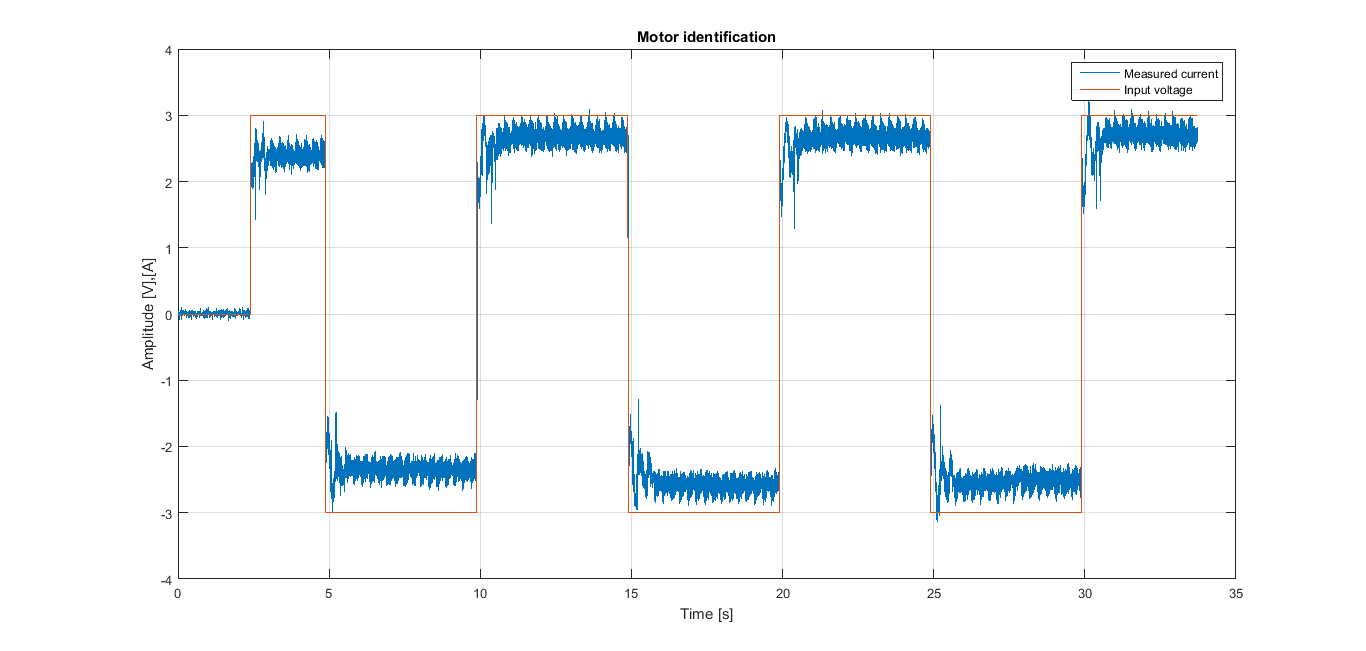
\includegraphics[width=0.5\textwidth]{img/motor_id_1.png}}
  \hfill
  \subfloat[Rising time of the current, it can be seen that steady state is approached very quickly.]{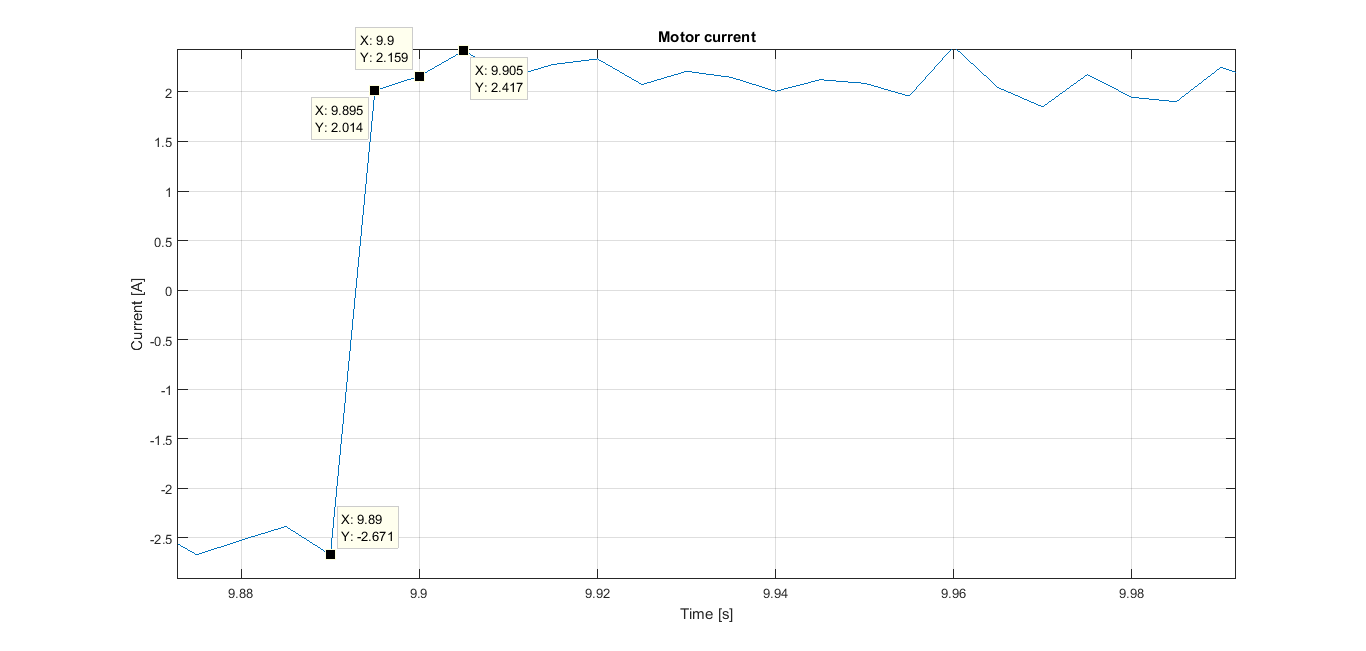
\includegraphics[width=0.5\textwidth]{img/motor_id_2.png}}
  \caption{}
    \label{fig:motorid}
\end{figure}
\subsection{Validation}
\label{sec:validation}
Validation was done using a random input with normal distribution $N(0,\frac{9}{4})$ (Check figure \ref{fig:motor_validation} ). Notice that we couldn't have used that input as source for identification because we already know a model of the system, and so we are not interested in black box modeling. 

On average, using the cost function defined in \ref{sec:validation_cost_function}, with a first order system of the type:
$$G(s) = \frac{1}{Ls+R}$$
where $R=1.2689 \Omega, L=0.0024 H$, there is an average fit value $d(i_{real},i_{sim})=0.8142$ with standard deviation $0.0364$.
\begin{figure}[!h]
    \centering
    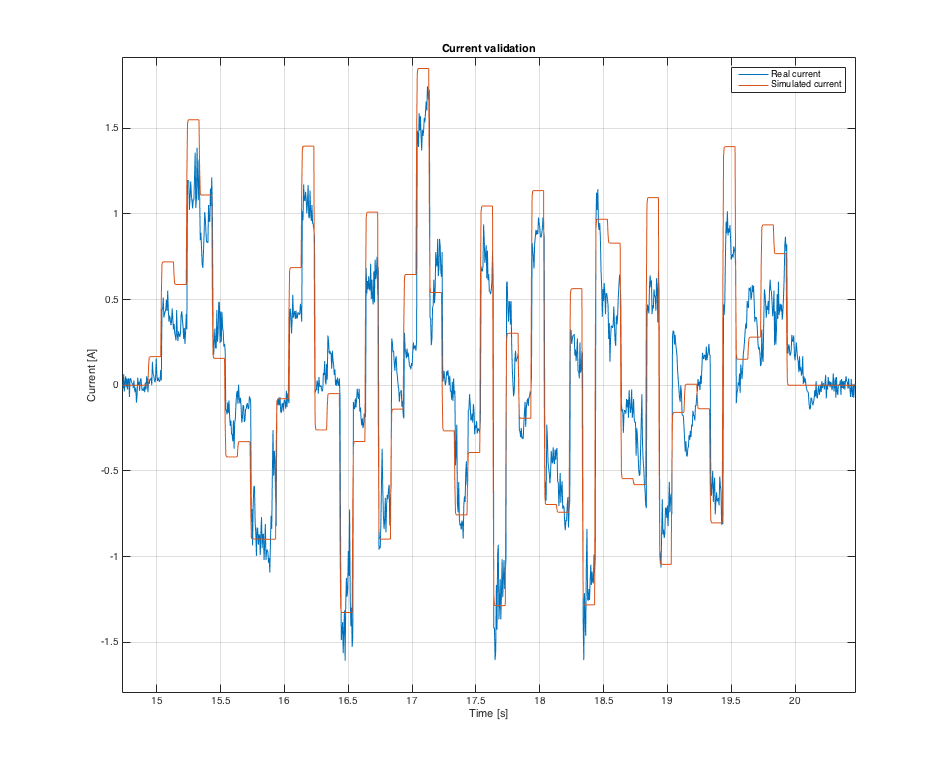
\includegraphics[width=0.5\textwidth]{img/motor_validation.png}
    \caption{Validation of the motor with a random input signal $v(t) \sim N(0,\frac{9}{4})$.}
    \label{fig:motor_validation}
\end{figure}
In case black box identification is used, with a $3$rd order system we would obtain an average fit value of $0.8527$ with standard deviation $0.0424$. \\ \\
\newpage
\section{Overall system identification}
The system was modelled as an open loop system as specified in section \ref{sec:validation_cost_function}.
We have mainly  a series connection of two systems: the motor and the cart, which are identified by the following transfer functions:

$$G_1(s) = \frac{1}{Ls+R} \quad G_2(s) = \frac{\gamma}{Ms^2+Cs+K}$$

Since we are using the same tests used to identify the motor (section \ref{sec:motor_id}), and the same techniques used to identify the cart detached from the motor (section \ref{sec:cart_detached_id}), those two sections are not presented.
\subsection{Experiment results}
Results are summarized in a similar fashion to section \ref{sec:cart_detached_id}:
\paragraph{Pulsation}
In the table below are shown the various mean of the pulsation of the cart and their relative standard deviation:
\begin{table}[!h]
\centering

\label{table: cart_attached_omega}
\begin{tabular}{|l|l|l|l|}
\hline
{(\textbf{$\omega_{avg}$} [\SI{}{\radian \per \second}],$\omega_{std}$ [\SI{}{\radian \per \second}])} & \textbf{$k_h$} & \textbf{$k_m$}   & \textbf{$k_l$}   \\ \hline
\textbf{with load}         & (20.2100, 0.0022)    & (13.0633, 0.3208) & (10.7500, 0.0308)      \\ \hline
\textbf{with no load}      & (30.4300, 0.2895)    & (18.3767, 0.2011) & (15.6240, 0.1820) \\ \hline
\end{tabular}
\caption{Pulsation of the cart  attached to the motor. Various configuration are shown (with a load of $0.986$ [\SI{}{\kilo \gram}] and no load) for the various springs. }
\end{table} \\ \\


\paragraph{System gain, mass and  stiffness}
By using   mean pulsation the resultant average mass of the system, including the cart, is $ 0.8906$ [\SI{}{\kilo\gram}] with standard deviation $  0.1146$ [\SI{}{\kilo \gram}]. Results also for the stiffness  are shown in table \ref{table: cart_springs_mass}.
\begin{table}[!h]
\centering
\label{table: cart_attached_springs_mass}
\begin{tabular}{|l|l|l|}
\hline
{\textbf{($k_h$ [\SI{}{\newton \per \metre}], $m$ [\SI{}{\kilo \gram}])}} & \textbf{($k_m$ [\SI{}{\newton \per \metre}], $m$ [\SI{}{\kilo \gram}])} & \textbf{($k_l$ [\SI{}{\newton \per \metre}], $m$ [\SI{}{\kilo \gram}])} \\ \hline
(720.56, 0.778)              & (340.14, 1.007)     & (216.38, 0.8864)     \\ \hline
\end{tabular}
\caption{Identified stiffness and mass of the overall system}
\end{table}
Therefore it results that the mass contribution of the motor is:
$$M_{motor} = 0.8906 -0.5685=0.3221 \text{Kg}$$.

The identified gain of the motor, based on the fact that at steady state we have:
$$x(\infty) = \frac{\gamma}{k} i(\infty)$$
gives an average value of $\gamma=  -2.0680$ \SI{}{\newton \per \ampere} and standard deviation $\gamma_{std}= 0.2935$ \SI{}{\newton \per \ampere}. Notice that $x(\infty), i(\infty)$ refers to the corresponding value at steady state.


\paragraph{Damping and damping ratio}
The mean values for the damping ratio, including their standard deviation, are shown in table \ref{table: cart_attached_dampingratio} for the various springs, with and without a load.
\begin{table}[!h]
\centering

\label{table: cart_attached_dampingratio}
\begin{tabular}{|l|l|l|l|}
\hline
{(\textbf{$\xi_{avg}$},$\xi_{std}$)} & \textbf{$k_h$} & \textbf{$k_m$}   & \textbf{$k_l$}   \\ \hline
\textbf{with load}         & (0.1356,  0.00022)    & (0.1949, 0.0080) & (0.2230, 0.0042) \\ \hline
\textbf{with no load}      & (0.1670, 0.0084)    & (0.2569, 0.0124) & (0.2973, 0.0376)      \\ \hline
\end{tabular}
\caption{Damping ratio. Various configuration are shown (with a load of $0.986$ [\SI{}{\kilo \gram}] and no load) for the various springs. }
\end{table}


From the values shown in table \ref{table: cart_attached_dampingratio} it seems that the damping $C$ is function of the mass, like in \ref{table: cart_detached_dampingratio}. The various damping values are shown in table 
\ref{table: cart_detached_damping}.
\begin{table}[!h]
\centering
\label{table: cart_attached_damping}
\begin{tabular}{|l|l|l|l|}
\hline
{$C$ [\SI{}{\newton \second \per \metre}]} & \textbf{$k_h$} & \textbf{$k_m$}   & \textbf{$k_l$}   \\ \hline
\textbf{with load}         &  10.2855    & 9.5558 & 8.9973 \\ \hline
\textbf{with no load}      & 9.0517 &    8.4089 &   8.2736      \\ \hline
\end{tabular}
\caption{Damping values. Various configuration are shown (with a load of $0.986$ [\SI{}{\kilo \gram}] and no load) for the various springs. }
\end{table}

We can therefore linearly characterize the damping value as function of the mass centered in $m_c$, for each spring:
$$C(m)=C_{nl}+ \frac{C_{l}-C_{nl}}{m_{l}}(m -m_{c}) = C_{nl} +\alpha (m-m_{c})$$
The different values of $\alpha$, the difference quotient, are shown in table \ref{table: cart_detached_damping_quotient}

\begin{table}[!h]
\centering
\label{table: cart_attached_damping_quotient}
\begin{tabular}{|l|l|l|l|}
\hline
 & \textbf{$k_h$} & \textbf{$k_m$}   & \textbf{$k_l$}   \\ \hline
$\frac{C_{l}-C_{nl}}{m_{l}}$ [\SI{}{\newton \second \per \metre \per \kilo\gram}]       &1.2514   & 1.1631 & 0.7340 \\ \hline
\end{tabular}
\caption{Damping difference quotient. Due to friction damping changes for different weights, we can therefore characterize the damping in a linear way with the formula: $C(m)=C_{nl}+ \frac{C_{l}-C_{nl}}{m_{l}}(m -m_{c})= C_{nl} +\alpha (m-m_{c})$. Values of the difference quotient are shown for the different springs.}
\end{table}

\subsection{Validation}
For the validation procedure we used the same input voltage used in the validation of the motor, section \ref{sec:validation}. $v(t) \sim \alpha N(0,\frac{9}{4})$, where $\alpha \in (0.7, 1.5)$ based on which spring was attached to the first cart. 
\subsubsection{Validation 1 DOF}
For each spring we made two tests, one without load and one with a load of about $1$\SI{}{\kilo\gram}, for a total of $6$ tests. \\Validation using only one cart can be summarised in an average fit value of $85.42$ \%, with standard deviation of $1.68$ \%. Because of such high value, there is no need to consider more details in the models such as back-emf or nonlinearities.\\ 
In figure \ref{fig:val_overall} some validation plots are shown.
\begin{figure} [!h]
\begin{minipage}[t]{0.4\textwidth}
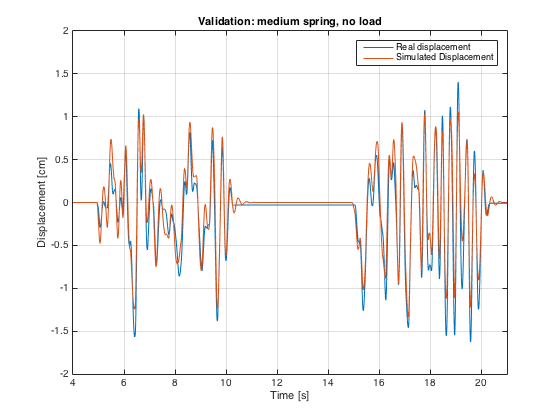
\includegraphics[width=\linewidth]{img/validation_overall_km_nomass.png}
\caption{Validation test without load and $K_m$.}
\label{fig:valov_1}
\end{minipage}
\hspace{\fill}
\begin{minipage}[t]{0.4\textwidth}
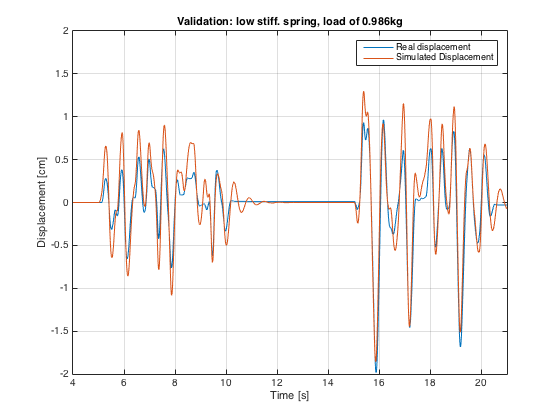
\includegraphics[width=\linewidth]{img/validation_overall_kl_2mass.png}
\caption{Validation test with load and $K_l$.}
\label{fig:valov_2}
\end{minipage}

\vspace*{0.5cm} % (or whatever vertical separation you prefer)
\begin{minipage}[t]{0.4\textwidth}
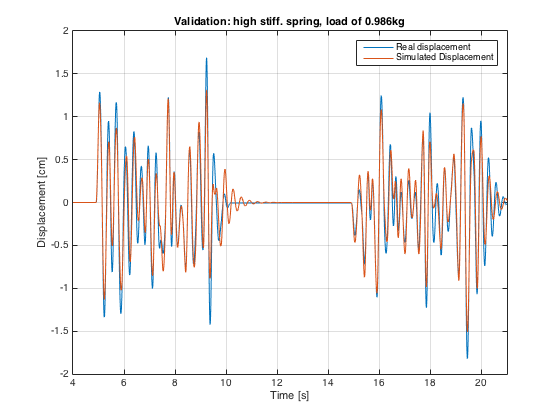
\includegraphics[width=\linewidth]{img/validation_overall_kh_2mass.png}
\caption{Validation test with  load and $K_h$.}
\label{fig:valov_3}
\end{minipage}
\hspace{\fill}
\begin{minipage}[t]{0.4\textwidth}
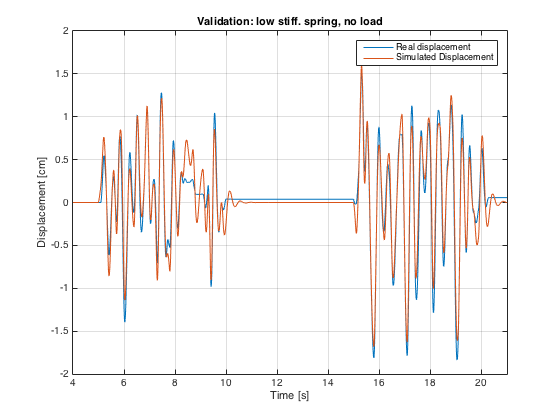
\includegraphics[width=\linewidth]{img/validation_overall_kl_nomass.png}
\caption{Validation test with  no load and $K_l$.}
\label{fig:valov_4}
\end{minipage}
\caption{Validation tests of the cart attached to the motor. In orange the simulated output, in blue the measurement of the validation test.}
\label{fig:val_overall}
\end{figure}
\subsubsection{Validation 2 DOF}
Validation for $2$ degree of freedom used the same random distribution of the validation input for $1$ degree of freedom. We tested the combination $K_h,K_m$ and $K_l,K_h$. For each combination we made $3$ tests, one without any load on the two carts, one with half kilogram on  each cart, and one with $1$ kilogram only on the second cart.\\ Since now we have $2$ outputs, the position of the first and second cart, we need to average the results for the first and second cart. \\ \\
For the first cart we have an average fit of $87.29$ \% with standard deviation $4.5$\%. For the second cart the average fit is $85.79\%$, with standard deviation $4.8$ \%.\\ This results in a mean of $86.54$ \%, and standard deviation $4.68$ \%. Some validation plots are shown in figure \ref{fig:val2dof} for the second cart.
\begin{figure} [!h]
\begin{minipage}[t]{0.4\textwidth}
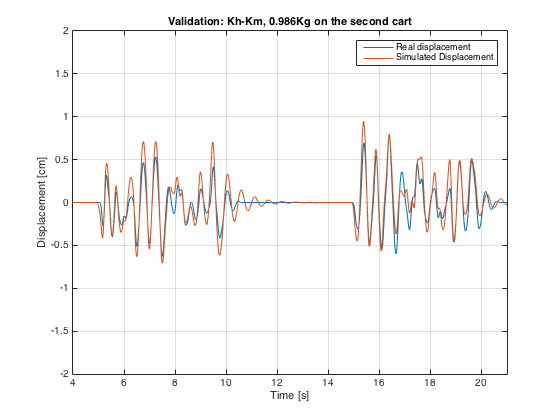
\includegraphics[width=\linewidth]{img/validation_overall_2dof_khkm_0m2m.png}
\caption{Validation test without load on the first cart, and a load of $0.986$\SI{}{\kilo \gram} on the second one. The configuration $K_h,K_m$ was used.}
\label{fig:valov_2dof1}
\end{minipage}
\hspace{\fill}
\begin{minipage}[t]{0.4\textwidth}
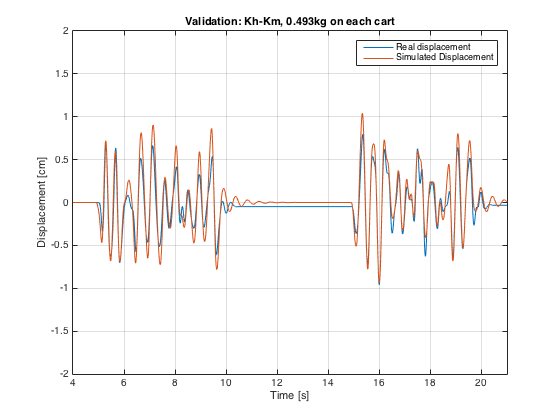
\includegraphics[width=\linewidth]{img/validation_overall_2dof_khkm_1m1m.png}
\caption{Validation test a load of about  $0.493$ \SI{}{\kilo \gram} on both the carts. The configuration $K_h,K_m$ was used.}
\label{fig:valov_2dof2}
\end{minipage}

\vspace*{0.5cm} % (or whatever vertical separation you prefer)
\begin{minipage}[t]{0.4\textwidth}
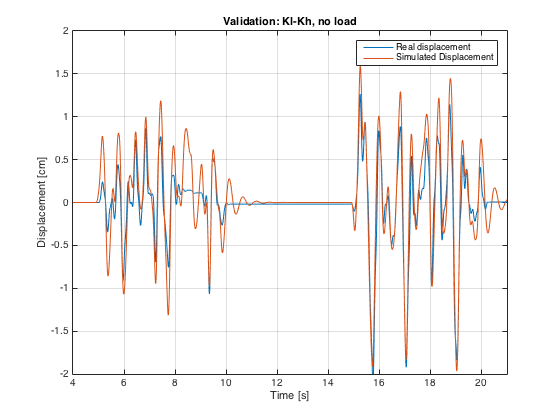
\includegraphics[width=\linewidth]{img/validation_overall_2dof_klkh_0m0m.png}
\caption{Validation test with no load on both the carts. The configuration $K_l,K_h$ was used.}
\label{fig:valov_2dof3}
\end{minipage}
\hspace{\fill}
\begin{minipage}[t]{0.4\textwidth}
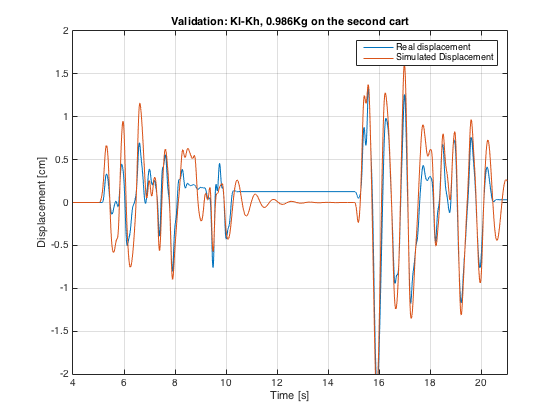
\includegraphics[width=\linewidth]{img/validation_overall_2dof_klkh_0m2m.png}
\caption{Validation test without load on the first cart, and a load of $0.986$\SI{}{\kilo \gram} on the second one. The configuration $K_l,K_h$ was used.}
\label{fig:valov_2dof4}
\end{minipage}
\caption{Validation tests of $2$ degree of freedom. Only the output for the second cart is shown. In orange the simulated output, in blue the measurement of the validation test.}
\label{fig:val2dof}
\end{figure}